\documentclass[a4paper,12pt]{article}
\usepackage{learnpackage}


\newcommand{\mkst}{\makebox[-3pt][r]{\color{blue}\ding{78}}}
\newcommand{\lbf}[1]{\kaishu\textbf{\color{cyan}#1}}
\newcommand{\lsn}[1]{\noindent\textsc{\color{orange} #1.}}
\newcommand{\lunl}[1]{\underline{\hbox to #1{}}}%%  可输入长度的下划线

\setlength{\headheight}{14.9998pt}
\addtolength{\topmargin}{-2.49998pt}

\pgfplotsset{compat=1.18}

%------------------Document----------------------------

\begin{document}

%-------------------------TitlePage------------------------
%\begin{titlepage}
%\end{titlepage}

%-------------------------Content------------------------
\section{动量一}
\subsection{动量定理}

\lsn{1}冲量定义：\lunl{10cm}

\lsn{2}动量定义：\lunl{10cm}

\lsn{3}动量变化量：\lunl{10cm}

\lsn{4}动量定理（文字及公式）：
\vspace*{2cm}

\lsn{5}推导动量定理：{\fangsong\footnotesize 如图所示，光滑地面上质量为\(m\) 的物块在恒力\(F\)作用下，速度由\(v_1\)变为\(v_2\)，时间为\(t\)，请推导动量定理。} 

\begin{tikzpicture}
  \draw[thick] (0,0)--(5.2,0);
  \draw[fill=orange!50] (.2,0) rectangle(.6,.4);
  \draw[->,font=\scriptsize] (.2,.5)--node[above]{\(v_1\)}(.6,.5);
  \node[font=\scriptsize] at(.4,.2){\(m\)};
  \draw[draw=gray,fill=orange!30] (4.2,0) rectangle(4.6,.4);
  \draw[->,font=\scriptsize] (4.2,.5)--node[above]{\(v_2\)}(4.6,.5);
  \draw[->,font=\scriptsize] (.6,.2)--++(.5,0)node[right]{\(F\)};
  \node[font=\tiny] at(2.5,1){{\kaishu 地面光滑}};
\end{tikzpicture}
\vspace*{2cm}

\lsn{6}初速度为\(v_1\)，末速度为\(v_2\)，画出\(\Delta v\)并算出大小：
\begin{figure}[htbp]
  \begin{tikzpicture}
    \begin{scope}[yshift=.56cm]
      \draw[->,font=\scriptsize,blue] (0,0)--node[above]{\(v_1 =\) \,\qty{2}{m/s}}(2,0);
      \draw[->,font=\scriptsize,red] (0,-.2)--node[below]{\(v_2 =\) \,\qty{1}{m/s}}(1,-.2);
    \end{scope}
    \begin{scope}[xshift=5cm,yshift=.6cm]
    \draw[->,font=\scriptsize,blue] (0,0)--node[above]{\(v_1 =\) \,\qty{2}{m/s}}(2,0);
    \draw[->,font=\scriptsize,red] (0,0)--node[below]{\(v_2 =\) \,\qty{1}{m/s}}(-1,0);
    \end{scope}
    \begin{scope}[xshift=10cm]
      \draw[->,font=\scriptsize,blue] (0,0)--node[below]{\(v_1 = v_2 =\) \,\qty{2}{m/s}}(2,0);
      \draw[->,font=\scriptsize,red] (0,0)--(120:2);
    \end{scope} 
\end{tikzpicture}
\end{figure}

\lsn{7}写出动量定理的应用流程，并应用于下图问题：{\fangsong\footnotesize 质量为\(m\)的小球从距沙坑高\(h\) 的位置静止落下，进入沙坑\(\Delta t\)时间后静止，求沙坑对小球的平均作用力。}
\begin{figure}[htbp]
  \begin{tikzpicture}
    \shade[ball color=blue!50] (0,1.5) circle(.1);
    \draw (-1,0)--(1,0);
    \draw[|<->|,font=\scriptsize,gray] (-.3,1.5)--node[black,fill=white]{\(h\)}(-.3,0);
  \end{tikzpicture}
\end{figure}
\vspace*{1.5cm}

\lsn{8}求高压水枪对墙面的冲击力：{\fangsong\footnotesize 水枪出水的速度\(v\)，出水的横截面积为\(S\)，水的密度为\(\rho\)}


\newpage
\subsection{动量守恒定律}
\lsn{1}动量守恒定律（{\kaishu 文字}）：
\vspace*{2cm}

\lsn{2}表达式：\lunl{20em}

\lsn{3}怎样区分内力和外力。
\vspace*{2cm}

\lsn{4}列出动量守恒的条件：
\vspace*{1cm}

\subsection{爆炸与反冲模型}
\lsn{1}基础模型：{\fangsong\footnotesize 如下图所示，质量为\(3m\)半径为\(R\)的光滑\(\frac{1}{4}\)圆弧轨道\(B\)静止在光滑的水平地面上，质量为\(m\)的小球\(A\)从轨道上静止释放，求小球\(A\)滑到水平面时\(A\)、\(B\)的速度\(v_1\)和\(v_2\)}
\begin{figure}[htbp]
  \begin{tikzpicture}
    \draw (0,0) arc(-90:-180:2)--++(-.2,0)--++(0,-2);
    \draw[dashed,cyan] (-2,2)--(0,2)--(0,0);
    \shade[ball color=blue!50,font=\scriptsize] (-1.9,2)node[above]{\(A\)} circle(.1);
    \foreach \x in {-2.4,-2.2,...,2}
      \draw[gray!50] (\x,-.2)--++(.2,.2);
    \draw (-2.4,0)--(2.2,0);
    \node[font=\scriptsize] at(-1.8,.4){\(B\)};
  \end{tikzpicture}
\end{figure}

\subsection{人船模型}
\lsn{1}基础模型：{\fangsong\footnotesize 如下图所示，质量为\(m\)的人站在质量为\(M\)的船上，船和人组成一个系统，假设水面光滑，船长为\(L\)。当人以速度\(v_1\)向右走时，求船的速度\(v_2\)及人从船的左端走到右端时人的位移\(x_1\) 和船的位移\(x_2\)}
\begin{figure}[htbp]
  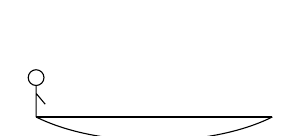
\begin{tikzpicture}
    \draw (0,0)--(3,0);
    \draw (0,0)..controls(.8,-.4)and(2.2,-.4)..(3,0);
    \draw (0,.5) circle(.1) (0,0)--(0,.4) (0,.3)--++(-50:.18);
  \end{tikzpicture}
\end{figure}

\end{document}